\documentclass[12pt]{article}
\usepackage{graphics}
\newcommand{\kg}{\mathrm{kg}}
\newcommand{\m}{\mathrm{m}}
\newcommand{\s}{\mathrm{s}}
\renewcommand{\deg}{\mathrm{deg}}
\newcommand{\km}{\mathrm{km}}
\newcommand{\cm}{\mathrm{cm}}
\newcommand{\mps}{\m\,\s^{-1}}
\newcommand{\mpss}{\m\,\s^{-2}}
\newcommand{\kgpmmm}{\kg\,\m^{-3}}
\newcommand{\N}{\mathrm{N}}
\newcommand{\J}{\mathrm{J}}
\newcommand{\Npmm}{\N\,\m^{-2}}
\newcommand{\tv}[1]{\mathbf{\vec{#1}}}
\newcommand{\dd}{\mathrm{d}}
\newcommand{\cell}[1]{\texttt{{#1}}}
\newcounter{problem}
\addtolength{\oddsidemargin}{-1in}
\addtolength{\textheight}{\headheight}
\setlength{\headheight}{0in}
\addtolength{\textheight}{\headsep}
\setlength{\headsep}{0in}
\setlength{\marginparwidth}{2in}
\begin{document}

\section*{NYU Physics 1---midterm exam}

Thursday 2009 October 15 in lecture.

\section*{Name:}

~ \vfill ~

\clearpage

\paragraph{Problem~\theproblem:}\refstepcounter{problem}%
The Moon is (1/80) the mass of the Earth.  If the compositions are
similar, what is the approximate radius of the Moon?  Give your answer
in units of $\km$.  State your assumptions and show your work
explicitly.

~ \vfill ~

\paragraph{Problem~\theproblem:}\refstepcounter{problem}%
In lecture we considered a car sliding around a banked circular turn
at constant speed, in the absence of friction.  Now imagine that the
car has static friction acting for transverse forces (that is,
opposing sliding up or down the bank) with a coefficient of $0.2$.
Draw the free-body diagram for the car---show only the forces and
their directions and approximate magnitudes---when it is going around
the turn at the maximum speed at which the car can go without sliding
uphill or downhill.  If you need to assume anything, state your
assumptions explicitly.

~ \vfill ~

\clearpage

\paragraph{Problem~\theproblem:}\refstepcounter{problem}%
Compute the velocity of the Space Shuttle in its orbit around the
Earth in units of $\mps$.  Show your calculation.  Assume the shuttle
is orbiting very close to the surface of the Earth (not a bad
approximation, as we discussed in class).  If you need to assume
anything else, state your assumptions explicitly.

~ \vfill ~

\paragraph{Problem~\theproblem}\refstepcounter{problem}%
A block of mass $m$ sits on an inclined plane, inclined at an angle
$\theta = 20\,\deg$ to the horizontal.  If the coefficient of friction
is $\mu = 0.9$ and the acceleration due to gravity is $g$, What is the
magnitude of the frictional force on the block, in terms of the
symbols given?  If you need to assume anything, state your assumptions
clearly.

~ \vfill ~

\clearpage

\paragraph{Problem~\theproblem:}\refstepcounter{problem}%
Imagine a particle of mass $m$ moving back and forth in the $x$
direction according to the equation
\begin{equation}
x(t)= A\,\cos\left(\omega\,t\right) \quad .
\end{equation}
What is the $x$-direction force as a function of time $F_x(t)$?

~ \vfill ~

\paragraph{Problem~\theproblem:}\refstepcounter{problem}%
What formulae should go into cells \cell{E9} and \cell{F9} in this
spreadsheet, which is integrating a trajectory?  State your formulae
in terms of the cell numbers (such as ``\cell{I8}''), not variables
(such as ``$a_x$''). \\
\resizebox{\textwidth}{!}{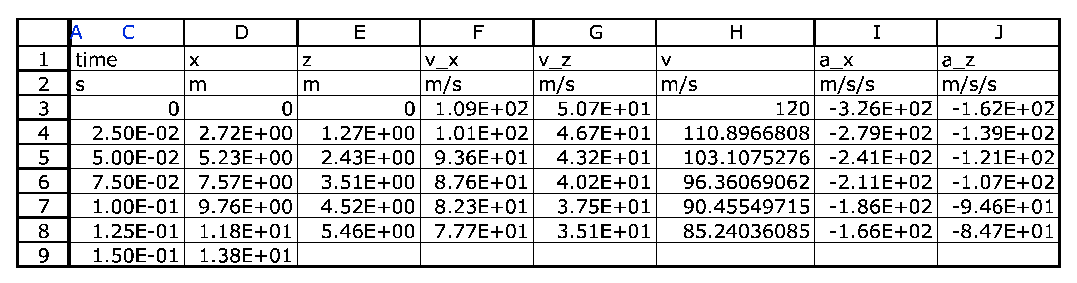
\includegraphics{../xls/exam.eps}}

~ \vfill ~

\clearpage

\paragraph{Problem~\theproblem:}\refstepcounter{problem}%
In lecture, I swung a full cup of iced tea in a vertical loop over my
head, like a roller coaster doing a loop-de-loop.  Explain, in
\emph{50 words or less} why the iced tea did not fall out when the cup
was upside-down.

~ \vfill ~

\end{document}
